% pacworld paper. Every number is read from the committed result files of the project repository.
\documentclass[11pt]{article}
\usepackage[margin=1in]{geometry}
\usepackage{amsmath,booktabs,graphicx,xcolor}
\usepackage[hidelinks]{hyperref}
\usepackage[numbers]{natbib}

\title{Hidden Timers and Context Offsets in a Diffusion World Model of Ms.~Pac-Man:\\
Pre-registered Tests and Replications}
\author{Sudish Mulakala}
\date{October 2, 2026}

\begin{document}
\maketitle

\begin{abstract}
Pixel diffusion world models predict the next frame from a few past frames, so they cannot see state the screen
does not show. We study a hidden timer in a DIAMOND-style model of Ms.~Pac-Man, whose ghosts wait in a pen for up
to 91 steps with no on-screen countdown. Models that see only their last 4 or 8 frames park the ghosts: in 450-step
rollouts on held-out episodes, 16--23 of 30 rollouts keep the pen occupied for 200+ steps, against none in the real
game. A 10-frame context with a 97-step reach removes the parking (0 of 30; paired difference to 4 frames $-0.57$,
95\% CI $[-0.77,-0.37]$ over episodes), and a pre-registered second training seed reproduces this. We propose a
context-offset hypothesis: a model can time a hidden event of period $N$ only as precisely as its context offsets
resolve $-N$. A
pre-registered sweep of 23 small models on a synthetic game, scored against an ideal observer with the same
offsets, supports it in part: no model times a period beyond its reach, a frame exactly $N$ steps back gives
observer-level timing at three of four long periods, and one period between two frames parks. Moving a single frame
from $-81$ to $-80$ takes that model from parking in 37 of 60 starts to none, in the original run and four further
training seeds. Several registered tests failed, among them the replication's second stage, a second real game, a
DIAMOND prediction and two latent-action models; all are reported.
\end{abstract}

\section{Introduction}
Diffusion world models generate convincing game frames from a short context of past frames and actions
\cite{alonso2024diamond,valevski2024gamengen}. The short context makes them blind to state the screen does not show.
Many games run clocks with no on-screen countdown. In Ms.~Pac-Man, ghosts wait in their pen for a fixed time after a
death, and a power pellet's effect lasts 124--134 steps. A model that sees only its last few frames cannot know how
long a ghost has been penned.

We make four contributions.
\begin{enumerate}
\item \textbf{A documented failure and a fix.} With a 4- or 8-frame context, our 18.8M-parameter diffusion model
parks ghosts in the pen. A strided context with a 97-step reach, a known design (Sec.~\ref{sec:related}), removes
the parking (Sec.~\ref{sec:context}).
\item \textbf{A testable hypothesis with an ideal-observer prediction,} and a pre-registered synthetic sweep in which
it holds in part (Sec.~\ref{sec:rule}).
\item \textbf{A one-variable follow-up} suggesting that timing depends on where the context frames sit, not only on how
far they reach. Moving one frame by one step fixes a parked period, in the original run and in all four seeds of a
pre-registered replication (Sec.~\ref{sec:followup}).
\item \textbf{A pre-registered evaluation that reports its failures:} a second real game that fails on timing
(Sec.~\ref{sec:realgame}), a failed prediction about DIAMOND (Sec.~\ref{sec:diamond}) and two failed latent-action
models (Sec.~\ref{sec:lam}). Confidence intervals are bootstrapped over held-out episodes.
\end{enumerate}
Sec.~\ref{sec:limits} lists the limits of the pre-registration and of the evidence.

\section{Setup}
\label{sec:setup}
\paragraph{Data.} \texttt{ALE/MsPacman-v5}~\cite{bellemare2013ale} with a 4-frame skip and max-pooling over all 4
frames. Ms.~Pac-Man draws one ghost per frame, and 2-frame pooling (the DQN default~\cite{mnih2015dqn}) shows all
four ghosts in only 29--47\% of observations. The maze crop of $172\times160$ pixels is area-resized to
$64\times64$. A PPO agent with $\varepsilon$-random and sticky-random exploration recorded 2.2M frames in 3,879
episodes. The validation split of 388 episodes is frozen by checksum.

\paragraph{Model.} An EDM~\cite{karras2022edm} denoising UNet with 18.8M parameters, widths 64/96/192/192 and
attention at 16 and 8 px. The noisy next frame is concatenated with the $K$ context frames; the actions enter
through adaptive group normalisation. Training uses GameNGen-style context-noise augmentation
\cite{valevski2024gamengen}; sampling uses 3 Euler steps. Training runs for 100k steps at learning rate
$10^{-4}$; where stated, a 15k-step anneal at $10^{-5}$ follows.

\paragraph{Context layouts.} The single variable of the ablation is the set of context offsets: \textbf{ctx4}
($-4..-1$), \textbf{ctx8} ($-8..-1$) and \textbf{ctx6s16} ($-97,-81,\dots,-17,-4..-1$: 10 frames, reach 97).

\paragraph{Evaluation.} Rollouts of 450 steps start at step 100 of the 10 longest held-out episodes, with 3 sampler
seeds each, and replay the recorded actions. Pixel detectors validated on real frames measure Pac-Man position
error, wall and pellet IoU, ghost count (gated by RAM), responsiveness (whether the model's Pac-Man turns where the
recorded action turns him) and pen occupancy (any non-background pixels in the pen box). Confidence intervals are
95\% bootstrap intervals over the 10 episodes with 10,000 resamples; a resampled episode keeps all three of its
seeds.

\section{The context ablation}
\label{sec:context}
\begin{table}[h]
\centering\small
\resizebox{\linewidth}{!}{%
\begin{tabular}{lcccc}
\toprule
model & parked 200+ steps & longest pen stay (median) & Pac-Man err @450 (px) & responsiveness @450 \\
\midrule
real game & 0/30 & 78 & -- & -- \\
Model 1 (4 frames, 200k data) & 16/30 [0.37, 0.70] & 222 [188, 299] & 19.5 [13.3, 25.4] & 0.30 [0.23, 0.38] \\
ctx4 (2.2M data) & 17/30 [0.37, 0.77] & 238.5 [150, 287] & 19.0 [13.2, 24.8] & 0.37 [0.28, 0.47] \\
ctx8 & 23/30 [0.63, 0.90] & 324 [282, 349] & 19.1 [12.6, 25.2] & 0.38 [0.26, 0.51] \\
\textbf{ctx6s16} & \textbf{0/30} [0, 0]$^*$ & \textbf{82} [73, 93] & 13.7 [9.1, 18.6] & 0.39 [0.36, 0.41] \\
ctx6s16 + LR anneal & 0/30$^*$ & 70 [65, 75] & 14.6 [10.4, 19.3] & 0.43 [0.40, 0.46] \\
ctx6s16, second seed & 0/30$^*$ & 104 [93, 107] & 17.8 [13.0, 23.1] & 0.38 [0.34, 0.42] \\
\bottomrule
\end{tabular}}
\caption{Pen-timer and coherence metrics at the 450-step horizon. Brackets: 95\% bootstrap CIs over episodes; for
parking, the CI of the parked fraction. All four originally reported pen numbers reproduce exactly. $^*$With no
parked rollout in any of the 10 episodes, the bootstrap interval is degenerate; the exact one-sided 95\% upper bound
on the per-episode parking rate is 0.26.}
\label{tab:context}
\end{table}

\paragraph{What holds.}
\begin{itemize}
\item The strided context removes the parking. The parked fraction falls by $-0.567$ $[-0.767,-0.367]$ against
ctx4, and by $-0.833$ $[-0.933,-0.733]$ in 900-step rollouts.
\item A second training seed reproduces this. We pre-registered one repeat of ctx6s16 from a new seed. It counts as
a replication if the CI of its paired difference to ctx4 lies below 0 and at most 3 of 30 rollouts park. It gave 0 of
30 parked and the same difference, $-0.567$ $[-0.767,-0.367]$. Timing is not exact in either seed: the new seed's
longest pen stay has median 104 and maximum 138 steps, against 78 and 91 in the real game.
\item The LR anneal improves responsiveness: $+0.044$ $[+0.009,+0.080]$.
\item Two significant differences among the 64px models at 450 steps are unfavourable. The strided context slightly
lowers wall IoU by $-0.007$ $[-0.011,-0.002]$ against ctx4, and by $-0.015$ $[-0.021,-0.009]$ in the second seed. Eight
consecutive frames lower pellet IoU by $-0.018$ $[-0.027,-0.010]$ against four.
\end{itemize}

\paragraph{What does not hold.}
\begin{itemize}
\item The claim that the strided context lowers Pac-Man error does not survive the second seed. The first seed
showed $-5.3$ px $[-11.6,-0.5]$ against ctx4; the second shows $-1.2$ px $[-6.7,+3.6]$, and the two seeds differ by
4.1 px $[+0.2,+8.1]$. We withdraw that claim.
\item There is no clear evidence that eight frames park more than four: $+0.20$ $[-0.10,+0.47]$.
\item There is no clear evidence that ten times more data changes parking ($+0.03$ $[-0.20,+0.27]$) or Pac-Man
error ($-0.5$ px $[-2.7,+1.3]$). Only responsiveness improves: $+0.071$ $[+0.014,+0.129]$.
\item No difference in ghost count between our models is significant. Ghost ratios at 450 steps are defined in only
4 of the 10 episodes (12 rollouts).
\item A $128\times128$ version is sharper per step but drifts faster: Pac-Man error $+8.2$ px $[+1.9,+13.9]$ in
64px-equivalent units.
\end{itemize}

\paragraph{The second timer is not solved.} The frightened timer of 124--134 steps exceeds the 97-step reach, and
no model ends frightened phases on time.
\begin{itemize}
\item A 145-step-reach model with 13 frames did not fix it. Of 15 phases, 8 never ended and none ended within
124--134 steps. It may also have weakened the pen timer that 10 frames had fixed: its median longest stay was 110.5
$[79, 136]$ against 82 $[73, 93]$, although the 97-step model's second seed gave 104 $[93, 107]$, so the gap is
within seed variation. It released fewer ghosts within 150 steps (cyan 62\% vs 97\%, pink 55\% vs 89\%; no paired
CI).
\item Oversampling training windows around phase ends did not fix it. In a matched pair fine-tuned on the same
enlarged data, with 25\% of each batch within $\pm8$ steps of a phase end, the 145-step model ended 23 of 25 phases
but too early: 2 of 19 scorable phases in range, median 84 steps. The 97-step model let phases run on: 0 of 9 in
range, phases ending after 61--611 steps (median 202), and 5 that never ended. An earlier oversampling run with the
97-step reach on the original data had 0 of 10 in range (5 early, 3 late, 2 never ended). The two parents of the
matched pair differ, since only the 97-step parent had an LR anneal, and each is one seed.
\item Teacher-forced analysis shows why. The models trained without oversampling (Model~1, ctx6s16 and the 145-step
model) copy the phase end one step after it appears in a real frame, 12 of 12 times, instead of predicting it. With
oversampling the lag fell to 0.6--0.8 steps, still above the registered bar of 0.5. The phase end is a one-frame
event that occurs 0.28 times per episode, about 0.05\% of training windows, which the denoising loss barely rewards.
\end{itemize}
Reach therefore appears necessary but not sufficient.

\section{The context-offset hypothesis}
\label{sec:rule}
\paragraph{Hypothesis.} An autoregressive frame model sees only its context. It can time a hidden-timer event of period
$N$ only as precisely as its context offsets resolve $-N$:
\begin{itemize}
\item exactly, if $-N$ is an offset;
\item spread over the gap, if $-N$ falls between two offsets;
\item not at all beyond the reach $R$. The best possible behaviour is then a geometric wait with hazard $1/(N-R)$,
and a sampling model may do worse by parking.
\end{itemize}

\paragraph{Ideal observer.} For each layout we estimate from training data the hazard
$P(\text{event next}\mid\text{state at the layout's offsets})$ and roll this observer out from the same test starts
as the models. It is the best that any model with those offsets can do, and its curve is the hypothesis's prediction. It
is computed and committed before any model trains.

\paragraph{Synthetic game.} Frames are $16\times16$. A ghost is penned for exactly $N$ frames, and nothing on screen
changes with elapsed time. The 23 cells cross three layouts with $N\in[3,200]$: C4 and C10 are consecutive with
reach 4 and 10, and S10 is ctx6s16's layout with reach 97. Each cell trains a small version of our model for 15k
steps. The pre-registered criteria require a model within reach to come close to the observer, and a model beyond
reach not to beat an observer blind to the capture.

\paragraph{Criteria.} R1 (exact offset in reach): on-time fraction at tolerance 2 $\ge\min(0.80,\text{ideal}-0.10)$.
R2 (gap in reach): release fraction $\ge\min(0.90,\text{ideal}-0.10)$ and median $|\text{lag}-N|\le$ ideal median
$+3$. R3 (out of reach, $N\ge1.5R$): on-time fraction at tolerance $\max(2,0.1N)$ $\le$ ideal $+0.15$. R4: at
$N\in\{33,65,97\}$, S10 passes R1 and C10 passes R3. The hypothesis holds if all pass, holds in part if every R3
cell passes but some R1 or R2 cell fails, and fails if any R3 cell fails. One R2 bar was amended before any model
trained, because the observer itself parks in the gap cells; the amendment is in the pre-registration.

\begin{table}[h]
\centering\small
\begin{tabular}{llccccc}
\toprule
cell & test & model on-time & ideal on-time & model release & ideal release & result \\
\midrule
C4 $N{=}3$ & R1 & 1.000 [1.000, 1.000] & 1.000 & 1.00 & 1.00 & pass \\
C10 $N{=}3$ & R1 & 1.000 [1.000, 1.000] & 1.000 & 1.00 & 1.00 & pass \\
C10 $N{=}8$ & R1 & 1.000 [1.000, 1.000] & 1.000 & 1.00 & 1.00 & pass \\
C10 $N{=}10$ & R1 & 1.000 [1.000, 1.000] & 1.000 & 1.00 & 1.00 & pass \\
S10 $N{=}3$ & R1 & 1.000 [1.000, 1.000] & 1.000 & 1.00 & 1.00 & pass \\
S10 $N{=}17$ & R1 & 0.867 [0.767, 0.950] & 0.901 & 1.00 & 1.00 & pass \\
S10 $N{=}33$ & R1 & 0.867 [0.767, 0.950] & 0.861 & 1.00 & 1.00 & pass \\
S10 $N{=}65$ & R1 & 0.817 [0.683, 0.917] & 0.801 & 1.00 & 1.00 & pass \\
S10 $N{=}97$ & R1 & 0.167 [0.067, 0.267] & 0.299 & 1.00 & 1.00 & \textbf{fail} \\
\midrule
S10 $N{=}8$ & R2 & 0.383 [0.283, 0.484] & 0.451 & 1.00 & 0.96 & pass \\
S10 $N{=}24$ & R2 & 0.317 [0.217, 0.433] & 0.326 & 0.82 & 0.89 & pass \\
S10 $N{=}80$ & R2 & 0.117 [0.050, 0.183] & 0.125 & 0.38 & 0.59 & \textbf{fail} \\
\midrule
C4 $N{=}8$ & R3 & 0.350 [0.217, 0.500] & 0.431 & 1.00 & 1.00 & pass \\
C4 $N{=}17$ & R3 & 0.067 [0.017, 0.133] & 0.139 & 0.65 & 1.00 & pass \\
C4 $N{=}33$ & R3 & 0.033 [0.000, 0.083] & 0.087 & 0.30 & 0.98 & pass \\
C4 $N{=}65$ & R3 & 0.033 [0.000, 0.083] & 0.077 & 0.28 & 0.94 & pass \\
C10 $N{=}17$ & R3 & 0.317 [0.233, 0.400] & 0.258 & 1.00 & 1.00 & pass \\
C10 $N{=}33$ & R3 & 0.117 [0.050, 0.183] & 0.109 & 0.73 & 0.99 & pass \\
C10 $N{=}65$ & R3 & 0.000 [0.000, 0.000] & 0.087 & 0.28 & 0.95 & pass \\
C10 $N{=}97$ & R3 & 0.017 [0.000, 0.050] & 0.082 & 0.17 & 0.93 & pass \\
C10 $N{=}200$ & R3 & 0.000 [0.000, 0.000] & 0.078 & 0.12 & 0.89 & pass \\
S10 $N{=}200$ & R3 & 0.017 [0.000, 0.050] & 0.146 & 0.23 & 0.96 & pass \\
\midrule
S10 $N{=}145$ & -- & 0.000 [0.000, 0.000] & 0.204 & 0.20 & 0.99 & unscored \\
\bottomrule
\end{tabular}
\caption{The synthetic hidden-timer sweep: 23 cells, 60 test starts in 20 test episodes each. On-time uses the
criterion's tolerance (2 for R1 and R2, $\max(2,0.1N)$ for R3 and the transition cell). Brackets: 95\% bootstrap
CIs over test episodes. The detector reproduces the true lag on every test start in every cell (D0). Point
estimates decide each criterion.}
\label{tab:timer}
\end{table}

\paragraph{Verdict: the hypothesis holds in part.}
\begin{itemize}
\item \textbf{No model times a period beyond its reach.} All 10 R3 cells pass. Instead of the observer's geometric
wait, the out-of-reach models mostly park: they release in 0.12--0.30 of starts at long periods (C4 $N\ge33$; C10
$N\ge65$; S10 $N{=}200$), against 0.89--0.98 for the observer. This reproduces the Ms.~Pac-Man pen parking in a game
with no other cause. R3 is one-sided: it shows that no model beat a blind observer, not that the models behave like
one.
\item \textbf{An exact offset gives exact timing when the observer is reliable.} All R1 cells but one pass. At S10
$N{=}17,33,65$ the model is within 0.04 of the observer, and at S10 $N{=}65$ the released lags have quartiles
65/65/65.
\item \textbf{Two in-reach cells fail.} At S10 $N{=}97$ the model is on time in 0.167 of starts against a bar of
0.199. The CI contains the bar, but point estimates decide. This was flagged before training as the weakest test in
the sweep: the $-97$ frame often falls inside the previous stay, so even the observer is on time in only 0.299. At
S10 $N{=}80$, a gap cell, the model releases near $N$ when it releases (lag quartiles 73/76/78.5) but parks in 37 of
60 starts. Its release fraction is 0.383 $[0.267, 0.500]$ against a bar of 0.494.
\item R4 holds at $N{=}33$ and $65$ and fails at $97$.
\end{itemize}
Reach is therefore necessary but not sufficient at this training budget. A gap, or a far offset that is often
masked, leads to parking or spread timing. That is a cost of striding.

\subsection{Follow-up: moving one frame}
\label{sec:followup}
The S10 layout has frames at $-81$ and $-65$, so $N{=}80$ falls between two frames, and that cell parked. We
pre-registered one follow-up before running it. The single change is the layout \textbf{S10b}: S10 with the frame
at $-81$ moved to $-80$, with the same reach, frame count, game, model, steps, seed, starts and scoring. The
registered prediction: the on-frame period $N{=}80$ passes R1, and the periods between frames of S10b ($N{=}72$, 79,
88) park, where parking means a release fraction below the R2 release bar.

This prediction differs from the original hypothesis, which said that between two frames the timing is spread over the
gap. The sweep instead showed parking at $N{=}80$, and the follow-up's prediction was registered after seeing that.
The follow-up therefore tests an explanation suggested by the sweep. The ideal observer, computed first, disagreed
in part: it releases in about 0.9 of starts mid-gap ($N{=}72$, 88) and in 0.59 at the end of a gap ($N{=}79$).

\begin{table}[h]
\centering\small
\resizebox{\linewidth}{!}{%
\begin{tabular}{llccccc}
\toprule
cell & $-N$ falls & on-time (tol 2) & release & ideal release & parked & result \\
\midrule
S10b $N{=}80$ & on a frame & 0.650 [0.533, 0.767] (ideal 0.716) & 1.000 & 1.000 & 0/60 & passes R1 (bar 0.616) \\
S10b $N{=}72$ & mid-gap & 0.233 & 0.783 [0.700, 0.867] & 0.898 & 13/60 & parks (bar 0.798) \\
S10b $N{=}79$ & end of gap & 0.117 & 0.350 [0.250, 0.450] & 0.594 & 39/60 & parks (bar 0.494) \\
S10b $N{=}88$ & mid-gap & 0.183 & 0.550 [0.417, 0.667] & 0.874 & 27/60 & parks (bar 0.774) \\
\bottomrule
\end{tabular}}
\caption{The follow-up: 60 test starts in 20 episodes per cell; brackets are 95\% bootstrap CIs over episodes.
Point estimates decide.}
\label{tab:followup}
\end{table}

\paragraph{Verdict: supported, as registered.}
\begin{itemize}
\item With the frame at $-81$, the $N{=}80$ model parked in 37 of 60 starts. With it at $-80$, it parks in none, and
its released lags have quartiles 80/80/81.
\item All three off-frame cells park. $N{=}79$ and $N{=}88$ fail clearly. $N{=}72$ fails by one start (47 of 60
released, 48 needed), and its CI contains the bar.
\item The observer predicted the ordering, with 79 worst, but the models park more than it does in every gap cell,
by 0.11 to 0.32.
\item Not every gap parks. In the main sweep the two short gap cells, S10 at $N{=}8$ and $N{=}24$, released in 1.00
and 0.82 of starts and passed R2. The replication below qualifies this.
\end{itemize}

\paragraph{Seed replication.} Every cell so far was trained once. We pre-registered a replication that changes only
the training seed: 18 new runs, with seed 0 as the original that does not count. Stage 1 repeats the headline pair
with seeds 1--4 and replicates if S10b $N{=}80$ passes R1 and S10 $N{=}80$ parks in at least 3 of 4 seeds each.
Stage 2 repeats five gap cells with seeds 1--2, three far from the recent frames (S10b $N{=}72, 79, 88$) and two
near them (S10 $N{=}8, 24$), and asks whether far gaps park in at least 5 of 6 runs while near gaps release in at
least 3 of 4.

\begin{table}[h]
\centering\small
\begin{tabular}{lccccc}
\toprule
 & seed 0 & seed 1 & seed 2 & seed 3 & seed 4 \\
\midrule
S10 $N{=}80$ (frame at $-81$): parked of 60 & 37 & 43 & 45 & 49 & 47 \\
S10 $N{=}80$: release (bar 0.494) & 0.383 & 0.283 & 0.250 & 0.183 & 0.217 \\
S10b $N{=}80$ (frame at $-80$): parked of 60 & 0 & 0 & 0 & 0 & 0 \\
S10b $N{=}80$: on-time (bar 0.616) & 0.650 & 0.650 & 0.700 & 0.733 & 0.717 \\
\midrule
S10b $N{=}72$: release (bar 0.798) & 0.783 & 0.633 & 0.667 & & \\
S10b $N{=}79$: release (bar 0.494) & 0.350 & 0.300 & 0.233 & & \\
S10b $N{=}88$: release (bar 0.774) & 0.550 & 0.600 & 0.400 & & \\
S10 $N{=}8$: release (bar 0.855) & 1.000 & 0.983 & 0.967 & & \\
S10 $N{=}24$: release (bar 0.791) & 0.817 & 0.733 & 0.533 & & \\
\bottomrule
\end{tabular}
\caption{Training-seed replication. Seed 0 is the original run. A gap cell parks when its release fraction is below
its bar. Point estimates; per-run 95\% bootstrap CIs are in Appendix~\ref{app:seeds}.}
\label{tab:seeds}
\end{table}

\begin{itemize}
\item \textbf{Stage 1 replicates, 4 of 4 for both claims.} With the frame at $-81$, every new seed parks in 43--49
of 60 starts (the original: 37). With it at $-80$, no seed parks in any start. The R1 pass is narrow in two of the
five runs (0.650 against 0.616); the absence of parking is not.
\item \textbf{Stage 2 does not hold as registered.} All 6 far-gap runs park, but only 2 of 4 near-gap runs release.
S10 $N{=}24$ parks in both new seeds, so its R2 pass in the main sweep, by two starts, does not replicate. The sweep
verdict is unchanged, but that cell is fragile.
\item A post-hoc summary, not a registered test: of the six gap cells trained with several seeds (S10 $N{=}80$ and
the five stage-2 cells), five park in most or all seeds. S10 $N{=}80$ and S10b $N{=}72, 79, 88$ park in every seed
and S10 $N{=}24$ in two of three. The exception is the nearest gap, $N{=}8$ between the frames at $-17$ and $-4$,
which releases in all three. The seed-1 miss at $N{=}24$ is narrow (0.733 against 0.791; its CI contains the bar).
\end{itemize}

\subsection{A second real game}
\label{sec:realgame}
\paragraph{Design.} The 2600 Pac-Man holds a ghost in its house for exactly 35 or 36 steps after every death. The
interval starts at a visible event, has no on-screen countdown, and is detectable at 64px in 622 of 622 held-out
stays. We recorded 1M steps of random play and trained the Ms.~Pac-Man recipe. The observer predicts a large
contrast: S10 on time in 0.889 of starts, C10 in 0.101. The registered criteria: pac-S10 must release in at least
0.898 of starts with a median timing error of at most 5 steps (P-S), and pac-C10 must not beat a blind observer
(P-C).

\paragraph{Attempt 1 stopped at its pilot.} A registered pilot required pac-S10, after 20k of 115k steps, to release
in at least 0.50 of starts. It released in 0.486 $[0.445, 0.525]$.

\paragraph{Attempt 2 failed on timing.} We registered the full run separately, with the same bars and with P-S as
the gate for training pac-C10. After 115k steps, pac-S10 releases in 0.986 $[0.976, 0.994]$ of starts and parks in 9
of 622, but its median timing error is 12 $[10, 13]$ steps against a bar of 5, and it is on time in 0.22
$[0.18, 0.25]$ of starts against the observer's 0.89. Its lags have 10th/25th/50th/75th/90th percentiles
28/33/44/72/96 against a truth of 35--36. P-S fails, pac-C10 was not trained, and the hypothesis is not confirmed on
this game. Before the 15k-step low-LR anneal, the same model released in only 0.678 of starts with a median error of 65.

\paragraph{A post-hoc reading.} The 35--36-step stay falls between S10's frames at $-33$ and $-49$. Loose timing and
parking between frames is what the synthetic follow-up found, so the failure is consistent with it. This reading was
made after the result and is not a registered test; no model with a frame at $-35$ or $-36$ was trained.

\section{External reference point: DIAMOND}
\label{sec:diamond}
\paragraph{What we ran.} DIAMOND released its trained Atari-100k Ms.~Pac-Man world model with a 4-frame context. We
ran it without retraining. We re-simulated our held-out episodes in its preprocessing, which includes the score area
and 2-frame pooling, and rebuilt our detectors for its geometry. All validity checks passed.

\paragraph{The registered prediction failed.} We had predicted that it would park ghosts in at least 10 of 30
rollouts. It parked in 0 of 30. The pre-registration stated that a failure with at least 5 of the model's own ghost
respawns ``counts against the rule'' (the pre-registration's term for the hypothesis); DIAMOND had 6. We report it
as a failed prediction that, by its registered terms, counts against the hypothesis, and we do not redefine the test.

\paragraph{A post-hoc reading.} The criterion assumed that ghosts survive long enough to be penned. Parking can only
be measured while ghosts exist, and DIAMOND's ghosts vanish (Fig.~\ref{fig:ghosts}). Its ghost count at 450 steps is
0.077 $[0.054,0.097]$ of its own ground truth, against 0.41 $[0.25,0.61]$ for our 4-frame Model~1 and 0.58
$[0.30,0.87]$ for our served model; these ratios are defined in 4 of the 10 episodes (12 rollouts). The vanishing is
not a detector artifact: over the first 15 steps the detectors find 0.99 $[0.97,1.01]$ of the ground-truth ghost
count in DIAMOND's generated frames, and 3.86 ghosts per ground-truth frame where 4 should be visible. We therefore
think the test says little about timing, but this argument was made after seeing the result.

\begin{figure}[h]
\centering
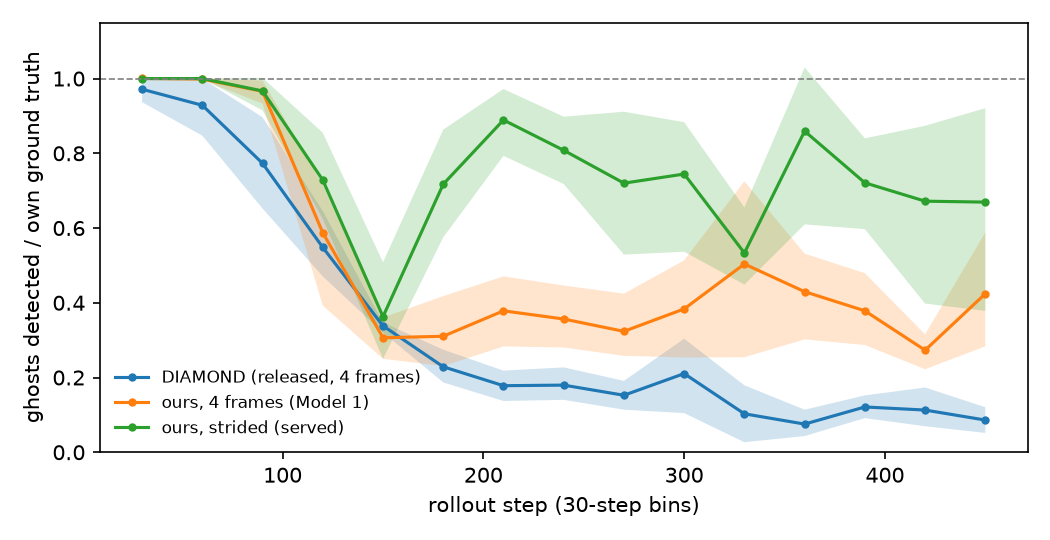
\includegraphics[width=0.75\linewidth]{ghost_ratio.png}
\caption{Ghosts detected in generated frames, relative to each model's own ground truth, over 450-step rollouts in
30-step bins. Bands: 95\% bootstrap CIs over the episodes whose ground truth shows ghosts in that bin (10 in the
first 60 steps, 3--9 after).}
\label{fig:ghosts}
\end{figure}

\paragraph{Other metrics.} DIAMOND keeps the walls best, with a wall IoU of 1.000 $[0.995,1.004]$ of its own
ceiling. It is worse on Pac-Man error (25.3 px $[19.1,31.2]$ over the 19 of 30 rollouts in which Pac-Man is still
detected, against 14.6 $[10.4,19.3]$ for our served model) and on responsiveness (0.18 $[0.13,0.24]$ against 0.43
$[0.40,0.46]$).

\paragraph{A reference point, not a head-to-head.} The two models differ in purpose (15-step imagination for RL
against long interactive rollouts), training data (100k steps of DIAMOND's own agent with episodes ending at each
life loss, against 2.2M frames of a PPO agent with exploration, about 20 times more), size (4.4M against 18.8M
parameters) and frame format (full screen with 2-frame pooling against a maze crop with 4-frame pooling). A
450-step rollout is 30 times DIAMOND's design horizon. The comparison measures long-horizon coherence, not the
merit of either design.

\section{Learned controls: two negative results}
\label{sec:lam}
\paragraph{Setup.} We trained a Genie-style latent action model~\cite{bruce2024genie} on frames only: 8 codes, a VQ
bottleneck~\cite{vandenoord2017vqvae} and a decoder built on the world model's UNet, under a label firewall tested
by double runs with scrambled labels. The loss is weighted around Pac-Man with a pixel detector; v1 also had an
unweighted arm.

\paragraph{v1: the decoder ignored the code.} With the 97-step context, both arms collapsed to one or two codes, and
the code gain (shuffled-code error over inferred-code error) was 1.000. The pre-registered stop fired before any
label was read.

\paragraph{v2: the collapse was fixed, but the codes captured the ghosts.} v2 changed five things, registered in
advance: a decoder that sees only the last frame, an entropy term on code usage~\cite{yu2024magvit2} with its weight
tied to the loss scale, non-zero initial code influence, a single player-weighted arm, and the code as extra input
channels. A 2,500-step pilot had three conditions. Perplexity was 7.42 (bar $\ge 4$, pass) and code gain 1.020 (bar
$>1.01$, pass). The third condition asked where the codes act: over 1,000 held-out contexts decoded with all 8
codes, the share of the output variance near Pac-Man had to exceed the share near ghosts. It was 0.067 near Pac-Man
against 0.400 near ghosts, and twice as large near ghosts per pixel. The pilot failed and the run stopped.

\paragraph{Mechanism.} The data come from a single recording agent whose moves are largely predictable from the
screen, so a code has little to add about the player. With a short decoder context, the ghosts are the largest
surprise in the next frame, and there are up to four of them, so the codes describe ghosts. No controllability
result exists for either version, and we have closed this line of work.

\section{Limitations}
\label{sec:limits}
\begin{itemize}
\item \textbf{Scope and seeds.} The main study uses one game, 64px frames and 10 evaluation episodes, hence the wide
CIs. Each training configuration has one seed, except the strided model (two seeds) and seven synthetic cells (the
four follow-up cells and S10 $N{=}8, 24, 80$ of the sweep, replicated with 2--4 further seeds); the other 20
synthetic cells were trained once.
\item \textbf{Limits of the pre-registration.} The first diagnosis of the parking was exploratory. The context
ablation had only an informal criterion, written before its result: pen stays should match the real game, with a
maximum of about 91 steps and no 200+ step runs. The no-200+ part held, but the strided model's longest stay was 148
steps. The follow-up's prediction was suggested by the sweep and registered before the follow-up's own runs. The
episode-level intervals were computed after the original runs, and several earlier claims did not survive them
(Sec.~\ref{sec:context}, ``What does not hold''). Many paired comparisons are reported without
correction for multiple comparisons, so intervals that barely exclude zero should be read with caution.
\item \textbf{The synthetic tests} isolate timing but have no action conditioning. Their out-of-reach criterion is
one-sided, so parking passes it. The follow-up is one layout with 60 starts per cell.
\item \textbf{The second real game} failed its registered test, and its C10 model was never trained, so the hypothesis
has no confirmation on a second real game. The strided run there was resumed once from the pilot's 20k-step checkpoint.
The learning rate (constant after warm-up), weights, EMA and optimizer state match an uninterrupted run, but the
batch and noise stream was re-seeded, so it is not bit-identical to one.
\item The frightened timer remains unsolved.
\item Responsiveness on replayed trajectories partly measures how predictable the agent is, not controllability.
\item The pen-occupancy measure is not resolution-invariant; at 128px its own ground truth differs.
\end{itemize}

\section{Related work}
\label{sec:related}
\paragraph{World models and neural game simulators.} World models were introduced for control
\cite{ha2018worldmodels,kaiser2019simple,hafner2023dreamerv3,micheli2023iris}. Learned simulators meant to be played
include GameGAN~\cite{kim2020gamegan}, whose memory module keeps revisited places visually consistent, and the
diffusion models DIAMOND~\cite{alonso2024diamond} and GameNGen~\cite{valevski2024gamengen}, on which our model is
based. These works evaluate visual quality, agent return or consistency when revisiting places. We evaluate whether
a hidden game clock is kept over hundreds of steps.

\paragraph{Memory and long context in video world models.} A growing line of work extends what a video model can
remember: training schemes for long rollouts and variable-length history
\cite{chen2024diffusionforcing,song2025history}, state-space and memory-bank architectures
\cite{po2025longcontext,xiao2025worldmem,lee2025edeline,savov2025statespacediffuser}, retrieval of relevant past frames
\cite{yu2025contextmemory,chen2025vrag}, and compressed or non-uniform history contexts
\cite{zhang2025framepack,gu2025far}. A context that mixes recent frames with sparser older ones is therefore not
new, and we do not claim the strided context as a contribution. These methods are evaluated mostly on spatial or
scene consistency. Closest to our question, Shin et al.~\cite{shin2026unobserved} show that standard video world
model architectures trained on short shell-game swap chains fail to track the hidden object's position on longer
chains, and that only architectures that carry a revisable state generalise. Related benchmarks and methods ask
whether hidden scene state keeps evolving out of view~\cite{ma2026stevo,duan2026liveworld}. To our knowledge, no
prior work studies elapsed-time tracking in a learned game simulator, relates timing accuracy to where the context
frames sit, or scores a model against an observer restricted to the same context offsets. Our search was not
exhaustive.

\paragraph{Partial observability.} A short stack of frames makes Atari only approximately Markov. Recurrent agents
were proposed as an alternative to frame stacking~\cite{hausknecht2015drqn}, and benchmarks isolate memory in agents
\cite{pasukonis2022memorymaze,morad2023popgym}. Convolutional sequence models reach long histories with dilated
convolutions~\cite{bai2018tcn}, an idea close to a strided context. Our contribution here is a measurement in a
generative world model, not a new memory mechanism.

\paragraph{Latent actions.} Genie~\cite{bruce2024genie} and LAPO~\cite{schmidt2023lapo} learn discrete latent
actions from video. Nikulin et al.~\cite{nikulin2025latent} show that such models degrade when the video contains
action-correlated distractors, and that a small amount of action supervision, 2.5\% of the data, improves them
substantially. Our second negative result, codes captured by the ghosts, is consistent with their finding and is not
a new failure mode. Our quantiser uses the entropy term of MAGVIT-v2~\cite{yu2024magvit2}.

\paragraph{Method.} Pre-registration for predictive modelling has been proposed as a guard against flexible
analysis~\cite{hofman2023preregistration}. We used it, with the limits stated in Sec.~\ref{sec:limits}.

\section*{Acknowledgments and AI-use disclosure}
The author used AI assistants (Anthropic's Claude) extensively to write code, run experiments, review designs and
results, and draft the text, including this paper. The author directed the project, set its rules
(pre-registration, budget limits and independent review), made the main research decisions, reviewed the results,
and takes full responsibility for the paper's contents. Within those rules, an AI reviewer approved designs and
results and chose some next steps. The experiments, pre-registrations and reviews are logged in the project
repository, \url{https://github.com/Sudish30/pacworld}.

\appendix
\section{Per-run intervals of the seed replication}
\label{app:seeds}
\begin{table}[h]
\centering\small
\begin{tabular}{llccccc}
\toprule
cell & seed & release [95\% CI] & release bar & on-time, tol 2 [95\% CI] & R1 bar & parked of 60 \\
\midrule
S10 $N{=}80$ & 0 & 0.383 [0.27, 0.50] & 0.494 & 0.117 [0.05, 0.18] & 0.025 & 37 \\
S10 $N{=}80$ & 1 & 0.283 [0.18, 0.38] & 0.494 & 0.083 [0.03, 0.15] & 0.025 & 43 \\
S10 $N{=}80$ & 2 & 0.250 [0.13, 0.37] & 0.494 & 0.050 [0.00, 0.10] & 0.025 & 45 \\
S10 $N{=}80$ & 3 & 0.183 [0.12, 0.25] & 0.494 & 0.083 [0.03, 0.15] & 0.025 & 49 \\
S10 $N{=}80$ & 4 & 0.217 [0.13, 0.30] & 0.494 & 0.083 [0.03, 0.15] & 0.025 & 47 \\
S10b $N{=}80$ & 0 & 1.000 [1.00, 1.00] & 0.900 & 0.650 [0.53, 0.77] & 0.616 & 0 \\
S10b $N{=}80$ & 1 & 1.000 [1.00, 1.00] & 0.900 & 0.650 [0.55, 0.75] & 0.616 & 0 \\
S10b $N{=}80$ & 2 & 1.000 [1.00, 1.00] & 0.900 & 0.700 [0.58, 0.82] & 0.616 & 0 \\
S10b $N{=}80$ & 3 & 1.000 [1.00, 1.00] & 0.900 & 0.733 [0.62, 0.83] & 0.616 & 0 \\
S10b $N{=}80$ & 4 & 1.000 [1.00, 1.00] & 0.900 & 0.717 [0.60, 0.83] & 0.616 & 0 \\
S10b $N{=}72$ & 0 & 0.783 [0.70, 0.87] & 0.798 & 0.233 [0.15, 0.33] & 0.217 & 13 \\
S10b $N{=}72$ & 1 & 0.633 [0.52, 0.75] & 0.798 & 0.150 [0.07, 0.23] & 0.217 & 22 \\
S10b $N{=}72$ & 2 & 0.667 [0.55, 0.77] & 0.798 & 0.167 [0.08, 0.25] & 0.217 & 20 \\
S10b $N{=}79$ & 0 & 0.350 [0.25, 0.45] & 0.494 & 0.117 [0.05, 0.18] & 0.020 & 39 \\
S10b $N{=}79$ & 1 & 0.300 [0.20, 0.40] & 0.494 & 0.083 [0.03, 0.15] & 0.020 & 42 \\
S10b $N{=}79$ & 2 & 0.233 [0.13, 0.35] & 0.494 & 0.067 [0.02, 0.13] & 0.020 & 46 \\
S10b $N{=}88$ & 0 & 0.550 [0.42, 0.67] & 0.774 & 0.183 [0.08, 0.28] & 0.154 & 27 \\
S10b $N{=}88$ & 1 & 0.600 [0.48, 0.70] & 0.774 & 0.200 [0.10, 0.32] & 0.154 & 24 \\
S10b $N{=}88$ & 2 & 0.400 [0.28, 0.50] & 0.774 & 0.133 [0.07, 0.20] & 0.154 & 36 \\
S10 $N{=}8$ & 0 & 1.000 [1.00, 1.00] & 0.855 & 0.383 [0.28, 0.48] & 0.351 & 0 \\
S10 $N{=}8$ & 1 & 0.983 [0.95, 1.00] & 0.855 & 0.367 [0.22, 0.52] & 0.351 & 1 \\
S10 $N{=}8$ & 2 & 0.967 [0.92, 1.00] & 0.855 & 0.350 [0.23, 0.48] & 0.351 & 2 \\
S10 $N{=}24$ & 0 & 0.817 [0.72, 0.90] & 0.791 & 0.317 [0.22, 0.43] & 0.226 & 11 \\
S10 $N{=}24$ & 1 & 0.733 [0.65, 0.82] & 0.791 & 0.267 [0.15, 0.38] & 0.226 & 16 \\
S10 $N{=}24$ & 2 & 0.533 [0.43, 0.65] & 0.791 & 0.150 [0.07, 0.25] & 0.226 & 28 \\
\bottomrule
\end{tabular}
\caption{Every run of the training-seed replication (Sec.~\ref{sec:followup}). Seed 0 is the original run. CIs are
95\% bootstrap intervals over the 20 test episodes. A gap cell parks when its release fraction is below its bar; the
on-frame cell (S10b $N{=}80$) is scored by R1. The same table is \texttt{results/supplementary\_results.md} in the
repository.}
\end{table}

\bibliographystyle{plainnat}
\bibliography{refs}
\end{document}
